% BEGIN TEMPLATE
\documentclass{article}
\usepackage{graphicx}
\usepackage{hyperref} 
\usepackage{xcolor}
\usepackage{nameref}
\usepackage{listings}
\usepackage{float}
\usepackage[title]{appendix}
\usepackage[ruled]{algorithm2e}
\graphicspath{ {../../images/} }
\bibliographystyle{acm}
% CHANGE THESE
\newcommand{\courseListing}{CSCI 8920}
\newcommand{\courseName}{Fundamentals of Deep Learning}
\newcommand{\assignmentTitle}{Homework Assignment \#2}
\newcommand{\assignmentSubtitle}{LeNet and Layers}
\usepackage{geometry}
\geometry{margin=1in}

\hypersetup{
    colorlinks,
    linkcolor={red!50!black},
    citecolor={blue!50!black},
    urlcolor={blue!80!black}
}
\urlstyle{same}
\definecolor{codegreen}{rgb}{0,0.6,0}
\definecolor{codegray}{rgb}{0.5,0.5,0.5}
\definecolor{codepurple}{rgb}{0.58,0,0.82}
\lstdefinestyle{mystyle}{
    commentstyle=\color{codegreen},
    keywordstyle=\color{magenta},
    numberstyle=\tiny\color{codegray},
    stringstyle=\color{codepurple},
    basicstyle=\ttfamily\footnotesize,
    breakatwhitespace=false,         
    breaklines=true,                 
    captionpos=b,                    
    keepspaces=true,                 
    numbers=left,                    
    numbersep=5pt,                  
    showspaces=false,                
    showstringspaces=false,
    showtabs=false,                  
    tabsize=2
}

\lstset{style=mystyle}

\begin{document}
  \begin{center}
  
\includegraphics[scale=0.15]{UNO-Logo-Color.png}
  \\[0.3in]
  \textbf{\courseListing{}}\\
  \courseName{}
  \\[0.75in]
  \textbf{\assignmentTitle{}}\\
  \assignmentSubtitle{}
  \\[0.75in]
  \textbf{Patrick Davlin}
  \\[0.75in]
  \textbf{Computer Science Department}\\
  \textbf{Peter Kiewit Institute}\\
  \textbf{University of Nebraska}
  \\[0.75in]
  \textbf{Spring 2021}
  \\[0.3in]
  
\includegraphics[scale=0.075]{UNO-Icon-Color.png}
  \newpage
\end{center}
  \graphicspath{{./images/}}
% END TEMPLATE
\section{Introduction}
Many deep learning programs with the Tensorflow framework also involve the use of Keras models.
The ability to use Keras effectively is enhanced by a more intimate knowledge of the components of a Keras model--its layers--and how those layers vary in importance to the model's capabilities.
This assignment represents a good basis upon which more understanding about Keras models can be developed, by implementing and examining the layers of a specific model, LeNet 5.
The structure of LeNet 5 is as follows:

\begin{figure}[H]
    \centering
    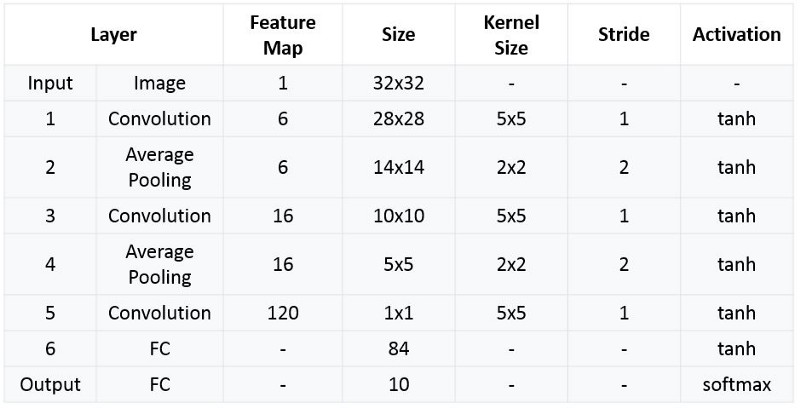
\includegraphics[width=6in]{csci-8920/hw-2/images/LeNet_structure.jpeg}
    \caption{LeNet structure table. Source: \href{https://www.datasciencecentral.com/profiles/blogs/lenet-5-a-classic-cnn-architecture}{Data Science Central}}
    \label{fig:lenet-table}
\end{figure}

The experiments performed on the developed model for this assignment were as follows:
\begin{itemize}
    \item Constructing the model in the Keras functional style, and graphing its accuracy and loss over time;
    \item Introducing varying magnitudes of noise at each layer, and evaluating the impact of that noise on the overall accuracy of the model; and,
    \item Allowing only one layer at a time to be trainable, to evaluate the impact of that layer on the overall accuracy of the model.
\end{itemize}

\section{Project Setup} \label{setup}
Similarly to Assignment #1, this assignment was done entirely on a local machine using the following specific packages:
\begin{itemize}
    \item Python 3.8.6 
    \item Tensorflow 2.4.1
    \item Matplotlib 3.3.4
\end{itemize}.

There is little else to say about the setup--with the Tensorflow tooling configured there is relatively little variation from assignment to assignment. 

\section{Implementation} \label{impl}
\textit{Note: this section discusses sections of code; the entire project can be found in the \nameref{codelist}}.
\subsection{Loading MNIST Data}
The first task for the assignment was to load and output MNIST data:
\begin{lstlisting}[language=Python]
# Load CIFAR10 data
(x_train, y_train), (x_test, y_test) = mnist.load_data()

# convert from uint to floats, and normalize to [0,1]
x_train = x_train.astype('float32')
x_test = x_test.astype('float32')
x_train = x_train / 255
x_test = x_test / 255

x_train = x_train.reshape(x_train.shape[0], 28, 28, 1)
x_test = x_test.reshape(x_test.shape[0], 28, 28, 1)

y_train = to_categorical(y_train, 10)
y_test = to_categorical(y_test, 10)


print('x_train.shape = ', x_train.shape, ' y_train.shape = ', y_train.shape)
print('x_test.shape = ', x_test.shape, ' y_test.shape = ', y_test.shape)

print('data type: ', type(x_train[0][0][0]))
print('label type: ', type(y_train[0][0]))

# plt.imshow(x_train[0], cmap='Greys')
plot_images(x_train)

# x_train = np.expand_dims(x_train, axis=-1)
\end{lstlisting}
To confirm, the resulting images are below:

\begin{figure}[H]
    \centering
    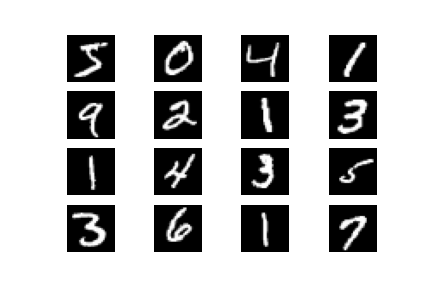
\includegraphics[width=3in]{csci-8920/hw-2/images/mnist.png}
    \caption{MNIST images}
    \label{fig:mnist}
\end{figure}

\subsection{LeNet Model}
Implementing the LeNet 5 model was a relatively straightforward procedure, since it simply involved adapting the \href{https://github.com/TaavishThaman/LeNet-5-with-Keras/blob/master/lenet_5.py}{Sequential Sample Code} provided in the assignment description.
This code was adapted to use the functional Keras construction, where the model is compiled as a function of inputs (the MNIST image data) and outputs (the result of a series of layer operations upon those inputs), as shown below:
\begin{lstlisting}[language=Python]
def LeNet_impl():

  data_in = keras.Input(shape=(28,28,1))
  kernel_size=(5,5)

  x = Conv2D(6, kernel_size, activation='relu', strides = (1,1), input_shape= (28,28,1), padding='same')(data_in)
  x = AveragePooling2D(pool_size=(2,2), strides = (2,2))(x)
  x = Conv2D(16, kernel_size, activation='relu', strides = (1,1))(x)
  x = AveragePooling2D(pool_size=(2,2), strides = (2,2))(x)
  x = Conv2D(120, kernel_size, activation='relu', strides = (1,1))(x)
  x = Flatten()(x)
  x = Dense(120, activation='relu')(x)
  x = Dense(84, activation='relu')(x)
  x = Dropout(0.5)(x)
  x = Dense(10, activation='softmax')(x)
  lenet_model = keras.Model(inputs = data_in, outputs = x, name = "lenet_model")
  lenet_model.compile(optimizer = 'SGD', loss = keras.losses.categorical_crossentropy, metrics = ['accuracy'])
  lenet_model.summary()
  return lenet_model
\end{lstlisting}

The \lstinline{model.summary()} result is shown below:

\begin{lstlisting}
Model: "lenet_model"
_________________________________________________________________
Layer (type)                 Output Shape              Param #   
=================================================================
input_1 (InputLayer)         [(None, 28, 28, 1)]       0         
_________________________________________________________________
conv2d (Conv2D)              (None, 28, 28, 6)         156       
_________________________________________________________________
average_pooling2d (AveragePo (None, 14, 14, 6)         0         
_________________________________________________________________
conv2d_1 (Conv2D)            (None, 10, 10, 16)        2416      
_________________________________________________________________
average_pooling2d_1 (Average (None, 5, 5, 16)          0         
_________________________________________________________________
conv2d_2 (Conv2D)            (None, 1, 1, 120)         48120     
_________________________________________________________________
flatten (Flatten)            (None, 120)               0         
_________________________________________________________________
dense (Dense)                (None, 120)               14520     
_________________________________________________________________
dense_1 (Dense)              (None, 84)                10164     
_________________________________________________________________
dropout (Dropout)            (None, 84)                0         
_________________________________________________________________
dense_2 (Dense)              (None, 10)                850       
=================================================================
Total params: 76,226
Trainable params: 76,226
Non-trainable params: 0
_________________________________________________________________
\end{lstlisting}

\\The model is then trained against the input MNIST data using the \lstinline{model.fit()} command as shown below:

\begin{lstlisting}[language=Python]
# default model run/train
model_default = LeNet_impl()
default_fitness = model_default.fit(x=x_train, y=y_train, steps_per_epoch=128, epochs=500, verbose=1, validation_data=(x_test, y_test))
model_default.save('./models/default')
with open('./histories/default/default.txt', 'w') as default_history_file:
    default_history_file.write(json.dumps(default_fitness.history))
\end{lstlisting}

For 500 epochs, as shown in this code, the results of the training can be visualized:

\begin{figure}[H]
\centering
\begin{subfigure}
  \centering
  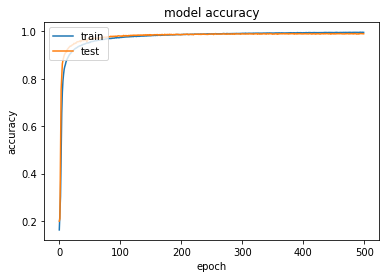
\includegraphics[width=3in]{csci-8920/hw-2/images/accuracy.png}
  \label{fig:accuracy}
\end{subfigure}%
\begin{subfigure}
  \centering
  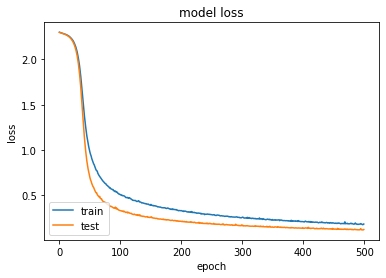
\includegraphics[width=3in]{csci-8920/hw-2/images/loss.png}
  \label{fig:loss}
\end{subfigure}
\caption{Results of LeNet 5 model after 500 epochs.}
\label{fig:default}
\end{figure}

From the outset it's obvious that 500 epochs with a batch size of 128 is much too high.
The model appears to stabilize before the 50th epoch.
The model can be re-run accordingly:

\begin{figure}[H]
\centering
\begin{subfigure}
  \centering
  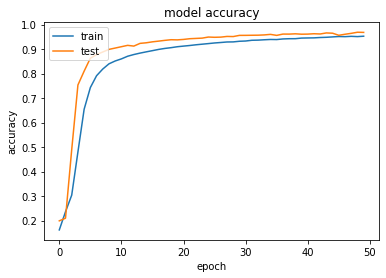
\includegraphics[width=3in]{csci-8920/hw-2/images/accuracy-50.png}
  \label{fig:accuracy-50}
\end{subfigure}%
\begin{subfigure}
  \centering
  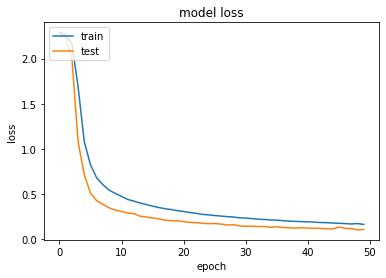
\includegraphics[width=3in]{csci-8920/hw-2/images/loss-50.png}
  \label{fig:loss-50}
\end{subfigure}
\caption{Results of LeNet 5 model after 50 epochs.}
\label{fig:default-50}
\end{figure}

Complete output supporting this is available in the \nameref{completeout} Appendix.

\subsection{Adding Noise} \label{kf}
The next step was to add noise to each layer and evaluate the results. 
This involved a slight adjustment to the model implementation.
Without having an effective way to quickly add noise to a layer, intermediate \lstinline{GaussianNoise()} layers were implemented in between layers as follows:

\begin{lstlisting}[language=Python]
def LeNet_impl(noise_layer = 0, noise_level = 1):

  data_in = keras.Input(shape=(28,28,1))
  kernel_size=(5,5)
  noise_level = noise_level / 100

  x = Conv2D(6, kernel_size, activation='relu', strides = (1,1), input_shape= (28,28,1), padding='same')(data_in)
  if noise_layer == 1:
    x = GaussianNoise(noise_level)(x)
  x = AveragePooling2D(pool_size=(2,2), strides = (2,2))(x)
  if noise_layer == 2:
    x = GaussianNoise(noise_level)(x)

  # ... and so on.
\end{lstlisting}

The Gaussian noise is adjustable, so several magnitudes were used in the a range between 0 and 2, in increments of 0.25.
The accuracy score at the end of 50 epochs (to remain consistent with the prior experiment) for each layer, at each noise magnitude, was plotted as follows:

\begin{figure}[H]
    \centering
    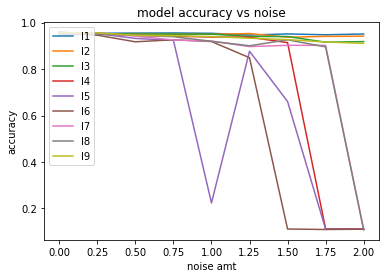
\includegraphics[width=3in]{csci-8920/hw-2/images/accuracy-noise.png}
    \caption{Accuracy $\times$ noise plot}
    \label{fig:mnist}
\end{figure}

This example is not as "pleasant" to look at as the finely colored and organized one provided in the reference paper from lecture notes.
Still, it is clear that some layers, like layer 4, 5, 6, and 8 were impacted more severely by the noise.
These layers correspond to the third \lstinline{Conv2D()} layer, the \lstinline{Flatten()} layer, the first \lstinline{Dense()} layer, and the \lstinline{Dropout()} layer.
It stands to reason, then, that these layers are of higher importance to the overall accuracy of the model.

Again, complete output supporting this is available in the \nameref{completeout} Appendix.

\subsection{Single-Layer Training}

The final task of the assignment was to organize the model such that only one layer would be trained at a time, with the remainder using the fixed weights as initialized.
To do this, the model was again adjusted to make one layer \lstinline{trainable} at a time, while others were fixed:

\begin{lstlisting}[language=Python]
def LeNet_impl_fixed(train_layer = 1, show_summary = False):
  """
  LeNet 5 implementation.
  """
  data_in = keras.Input(shape=(28,28,1))
  kernel_size=(5,5)

  x = Conv2D(6, kernel_size, activation='relu', strides = (1,1), input_shape= (28,28,1), padding='same', trainable=(train_layer == 1))(data_in)
  x = AveragePooling2D(pool_size=(2,2), strides = (2,2), trainable=(train_layer == 2))(x)
  
  # ... and so on.
\end{lstlisting}

Again, a loop of the model was run such that accuracy and loss could be evaluated as each layer was trained.
The layers were observed and evaluated after 50 epochs:

\begin{figure}[H]
\centering
\begin{subfigure}
  \centering
  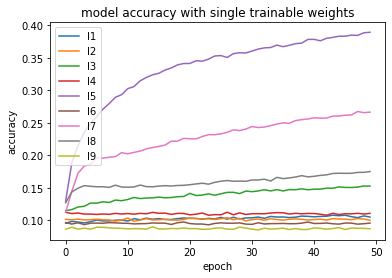
\includegraphics[width=3in]{csci-8920/hw-2/images/accuracy-trainable.png}
  \label{fig:accuracy-t}
\end{subfigure}%
\begin{subfigure}
  \centering
  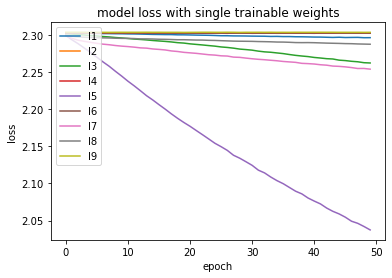
\includegraphics[width=3in]{csci-8920/hw-2/images/loss-trainable.png}
  \label{fig:loss-t}
\end{subfigure}
\caption{Results of training individual LeNet 5 model layers after 50 epochs.}
\label{fig:trainable}
\end{figure}

The results of this experiment line up well, generally, with the noise experiment.
The layers that most improved the overall with training were 3, 5, 6, and 7, corresponding to the second \lstinline{Conv2D()} layer, the final \lstinline{Conv2D()} layer, the \lstinline{Flatten()} layer, and the first \lstinline{Dense()} layer.
This suggests that, in terms of training, these layers are more valuable.

Extrapolating generally, since layers 5 and 6 were improved in both experiments, it could be concluded that these two layers are most vital to the LeNet 5 model.

\section{Conclusions}
The experiments run in the course of this assignment were valuable in encouraging more careful thought about the layers that compose Keras models.
In past assignments, these were composed as rote functions and easily taken for granted; having an opportunity to examine and discuss them further has encouraged me to evaluate models which might compose my own future projects.

\newpage
\begin{appendices}
\section{Complete Code Listing} \label{codelist}
\lstinputlisting[language=Python]{hw-2.py}
\end{appendices}
\end{document}